\section{Research Plan} 
\label{sec:research}

Visualizing the data from bike-share systems of a certain area can help us find many trends in the way this service is being used by the general public. What this project is primarily aiming for is to map the data to possibly find patterns and trends that can help us analyze the effectiveness of the bike-sharing system. The term effectiveness carries a broad meaning and needs to be narrowed down for the scope of this project. By creating visualizations that map bike-shared data with seasons, city congestion and subsequent daily revenues, we can reason about how effective the location of bike-stations are and about the sustainability of this service overall. As per out current milestone, no new visualizations or libraries have been planned. This is subject to change and further development into the project might bring about some new visualization as well. 

In an effort to develop data visualizations for the bike-share systems, we aim to create 3-4 visualizations, each handling a separate analysis of the data. Referencing Section~\ref{sec:intro}, we can see the list of visualizations which we will be working on. For the geographical visualizations, we plan on overlaying the data of each visualization category to the same geographical map with the user having a UI interface to switch between the various types of visualizations. Each category begs its own analysis, hence multiples topics/issues will be covered along the way of this project.
\begin{figure}[h]
	\centering % avoid the use of \begin{center}...\end{center} and use \centering instead (more compact)
	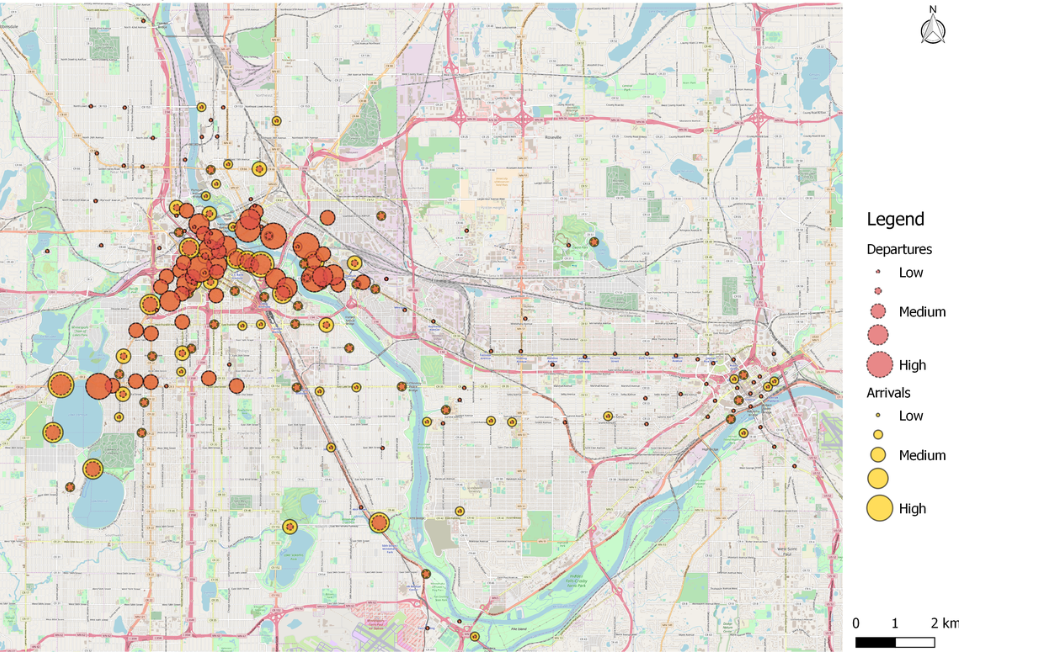
\includegraphics[width=1.5in]{figs/Heat}
	\caption{Extracted from a similar project which shows the user heatmap categorized by arrivals and departures.}
	\label{fig:Heat Map}
\end{figure}
Additionally, some bar charts to denote the revenue/running cost comparison will be introduced for sustainability analysis of this service. One possible hurdle for the near future can be the availability of initial budget and current running cost of the bike-share systems in LA. We do not have that data right now but hope to find it sooner. In the case that we are not able to find this data, we might have to perform an estimation from the budget cost of some other state whose data is available. For the worst case, we will discard this visualization for another similar one (yet to be decided).
\begin{figure}[h]
 \centering % avoid the use of \begin{center}...\end{center} and use \centering instead (more compact)
 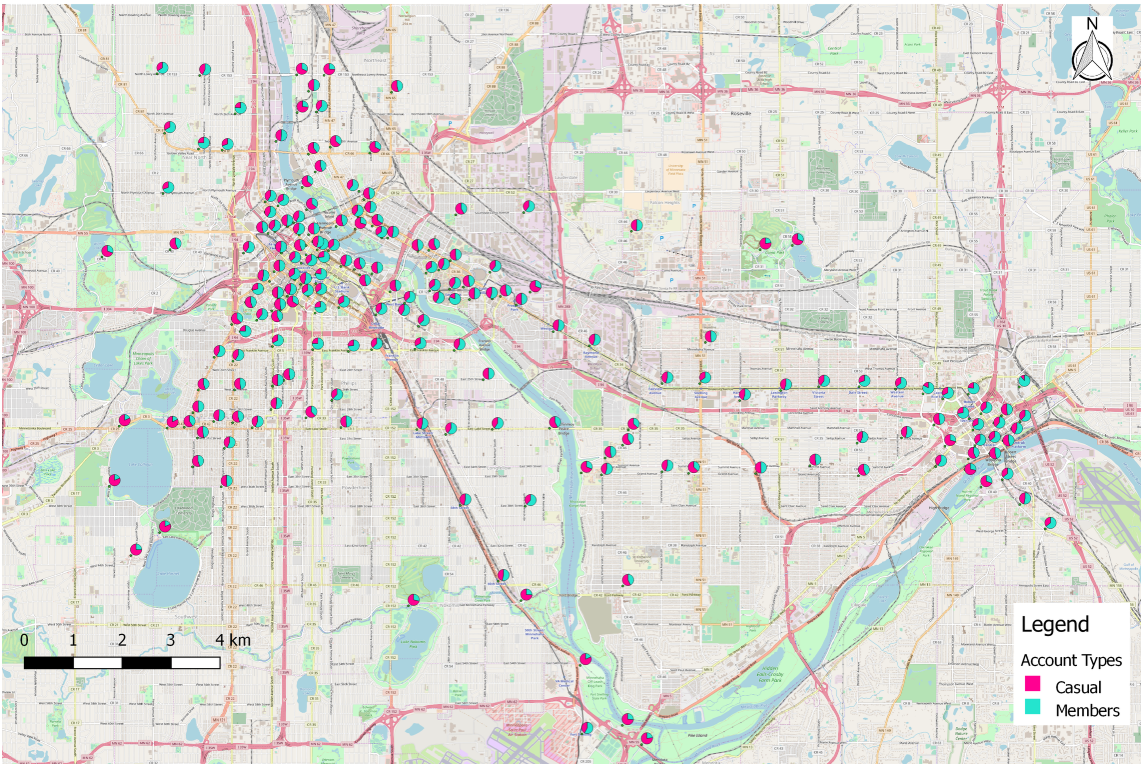
\includegraphics[width=1.5in]{figs/UserType}
 \caption{Extracted from a similar project which shows the categorization by customer type (Casual/Member).}
 \label{fig:Customer Type}
\end{figure}

\subsection{Data}
\label{sec:data}

% Describe the data here. Describe whether you already have access to the data
% and if not, what is required to obtain the data. If you don't already have the
% data, explain how long it will take to retrieve it. 

We initially obtained our data from a popular online data source, Kaggle. The dataset was named \textit{Los Angeles Metro Bike Share Trip Data}. Even though this dataset had enough depth to reason about various trends and patterns, it was less in number which made us look for other sources of similar data. We then found a substantial amount of data in Bike Share Metro, which seemed to fulfill our requirements for this project. This data, like the one before, is from Los Angeles and contains the shared bike ride information for 2.5 years, 2016 Q3 to 2018 Q2. Data is divided by quarters and contains the following fields:
\begin{itemize}
	\item trip\_id - Unique ID for a particular trip
	\item duration - Duration of trip in minutes
	\item start\_time - Start time of the trip
	\item end\_time - End time of the trip
	\item start\_lon - Starting position longitude
	\item start\_lat - Starting position latitude
	\item start\_station - The station ID where the trip originated
	\item end\_station -  The station ID where the trip terminated
	\item end\_lat - Destination latitude
	\item end\_lon - Destination longitude
	\item bike\_id - Id for each bike
	\item plan\_duration - Duration of the customers plan
	\item passholder\_type - The name of the passholder's plan
	\item trip\_route\_category\ -  "Round Trip" for trips starting and ending at the same station or "One Way" for all other trips
\end{itemize}
s
However, we do not currently know the budget required to setup this bike share system in a city. If we are to find this value, we can visualize cost vs revenue to help us calculate the sustainability of these services.
\subsection{Evaluation}
\label{sec:eval}

Describe your plan for evaluating your work during this project.

The dataset used in this project is completely based on the city of Los Angeles. So, though our visualization may point to certain trends, it is also possible that other factors are not taken into account which may affect adversely if the same model is implemented for other metro cities. Such as, the city of New York has a robust public transport system, which may have an adverse impact on the number of customers if the same business model as used in Los Angeles. So, given time it is possible to collect similar data from other cities for evaluation purpose which can give deeper insights into this matter.




\subsection{Technology}
\label{sec:tech}

% Describe what technologies you intend to use (e.g., programming languages,
% platforms, existing libraries) and why they make sense for your project. Do
% they serve your users better than other technologies? Are you able to take
% advantage of existing work/libraries for your domain with this technology
% rather than HTML/CSS/JS and d3js?  

For this project, we will be developing on HTML/CSS/Javascript as the primary programming languages. In terms of libraries, we will be using d3js. With all three team members being new to programming in d3js, we are not yet fully informed about its limitations. If, during the course of this project we find that d3js does not provide us with a specific functionality that we require, additional libraries might be used. For now, this choice of language and library makes sense because our visualization is not complex or novel. Most of our visualizations will be geographical maps and bar charts of varying types and our choice of programming language and libraries will be able to handle them well. 
In terms of user experience, our visualizations will provide users with seamless navigation and scrolling between various visualizations. Different data from different visualizations will be overlayed on top of a geographical map of LA. Users will be able to switch between various visualizations easily. D3js and JS will be able to handle this functionality hence serving the users pretty well. 
Since the concept of this project and the visualizations used on it have been worked on previously, several libraries such as TopoJSON, GeoJSON and Open Street API do exist. Using these libraries during various stages of the research will be very helpful as compared to just using HTML/CSS/JS and d3js. These libraries will be used during the initial data parsing and cleaning stage for sanity checks. Managing the data such that it will be easier to read through it during the visualization task is very important. Use of methods and techniques implemented in previous work/libraries will also come in handy but that area has not been looked into as of now. As the project advances, more idea about previous work on this topic will be gained which in turn will make us make this decision in a more refined manner than now.

\subsection{Timeline}
\label{sec:timeline}

Adapt the milestones for the class project to the specifics of your project
and summarize in Table~\ref{tab:milestones}.

The expectations are as follows:

\vspace{1.5ex}\noindent\textbf{Project Milestone Two} should include any task
and data abstraction necessary to support the project design whether it is
designing a user study, designing a new visualization, or designing a new
library. Initial designs should be included with discussion of the rationale
in support of the design. Data supporting all of these findings in terms of
background work or newly collected data (e.g., interviews, observations)
should be cited or discussed. 

Additionally, the related works should be updated with a more thorough
literature review. Changes to the status of the data and the choices of
technology should be discussed.

\vspace{1.5ex}\noindent\textbf{Project Milestone Three} should include the
results of the first chunk of work that needs to be done. In most projects
this will involve a working data reader and at least one visualization,
library feature, or study question type working. The milestone should include
images of these features and a discussion of what they do. The demonstration
should run with minimal effort and the code should be included in the
repository.

In the corresponding report, discussion of project progress as well as any
revisions to the data, technology choice, and scope should be included.

\vspace{1.5ex}\noindent\textbf{Project Milestone Four} should include a
complete working prototype of the main project artifact, such as a
visualization tool, a visualization library, or a working study with
experimental objects and stimuli complete. The demonstration should run with
minimal effort and the code should be included in the repository.

In the corresponding report, discussion of project progress as well as any
revisions to the data, technology choice, and scope should be included. The
plan for evaluation especially should be updated indicating the plan for
milestone five and any preliminary work in the design of that evaluation.


\vspace{1.5ex}\noindent\textbf{Project Milestone Five} should include initial
evaluation of the work from project milestone four and recommendations for
improvement. It will also include an in class presentation scheduled several
weeks before the report it due. Artifacts generated (e.g., pre-observation
plan, observation notes, data from studies) during this evaluation should be
included in the repository.

Additionally, a full report of the project as a whole should be included in
this milestone.



\begin{table}[h]
%% Table captions on top in journal version
 \caption{Project Milestones}\vspace{1ex} % the \vspace adds some space after the top caption
 \label{tab:milestones}
 \scriptsize
 \centering % avoid the use of \begin{center}...\end{center} and use \centering instead (more compact)
   \begin{tabular}{r|r}
     Milestone & Description (\%)\\
   \hline
     PM2 & Finalize on the dataset for visualization\\
     	 & Perform data cleansing and abstractions, categorizing them in the order in which they are mapped\\
         & Discuss and agree on detailed work division for the project\\
         & Perform initial visualization sketches\\
         & Decide on the feasibility of current visualization ideas and add/remove as required\\
     PM3 & Loaded geographic data into the visualization, creating the overlay for the mapping\\
         & First visualization mapping the busiest locations in the city complete\\
         & Initial work on panning and zooming started\\
         & Data analysis for feasibility study commenced\\
     PM4 & All visualization designs created and fully working\\
	 & Refined the interactions within a visualization\\
	 & Initial work on mechanisms for switching between visualizations\\
	 & Select data and mechanisms for evaluation\\
	 & Started preparations for class presentation\\
     PM5 & Evaluation process started with initial evaluation data\\
         & Revised data analysis and visualization tuning because on evaluation review\\
         & Class presentation and report submission completed\\
   \end{tabular}
\end{table}

